\subsection{Controller}

\begin{figure}[H]
\centering
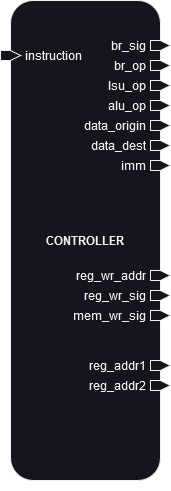
\includegraphics[width=0.35\textwidth]{../diagrams/decode/controller.png}
\caption{Diagram of the Controller}
\label{fig:controller}
\end{figure}

The controller is the main module of the ID stage. It is responsible for decoding the current instruction which is the action
of extracting the different fields of the instruction and forwarding them to the next stage. For more information about the different
types of instruction and how the data is encoded in the instruction, please refer to the RISC-V manual~\cite{riscv_manual}. \\

Signals:
\begin{enumerate}[label={\textbullet}]
    \item Input: $instruction$, This signal is representing the current instruction that is being decoded.
    \item Output: $br\_sig$, This signal is representing the state of the current instruction. 
    It is used to know if the instruction is a branch or not.
    \item Output: $br\_op$, This signal is representing the type of branch that is being executed.
    \item Output: $lsu_op$, This signal is representing the type of load or store that is being executed.
    \item Output: $alu\_op$, This signal is representing the type of ALU operation that is being executed.
    \item Output: $data\_origin$, This signal is representing the origin of the data that is being used by the ALU.
    That could be the registers, or one register and an immediate or one register and the PC.
    \item Output: $data\_dest$, This signal will be useful in the write-back stage to know which data to write back,
    so either the ALU result or the data from the memory or the next PC (so the PC+4).
    \item Output: $imm$, This signal is representing the immediate value that is being used by the ALU.
    \item Output: $reg\_wr\_addr$, This signal is representing the register address that will be written back.
    \item Output: $reg\_wr\_sig$, This signal is representing if we want to write to the register file or not.
    \item Output: $mem\_wr\_sig$, This signal is representing if we want to write to the memory or not.
    \item Output: $reg\_addr1$, This signal is representing the first register address that has been extracted from the instruction.
    \item Output: $reg\_addr2$, This signal is representing the second register address that has been extracted from the instruction.
\end{enumerate}